\chapter{Differential analysis of the NN output}
%\chapter{Analysis of the effects of different event features on the neural network output}
\section{Weighted correlations of input features with the NN output}

\subsection{Motivation for calculating correlations}
Correlations between input variables and the neural network's provide an overview of what the NN has "learned". 
They represent which input variables have the strongest influence on the output of the NN. 
The level of influence of any input variable is determined during the training phase of the NN. For example, suppose the value of a specific input variable turns out to be an essential parameter in the discrimination of the signal from the background. 
In that case, this variable will acquire a strong correlation after the training process. 
Consequently, strongly correlated variables would provide a critical basis to determine which properties of the $tq\gamma$ process help in understanding the photon to top quark coupling.  \\

\subsection{Steps of calculation}

Weighted correlations between two sets of data are calculated by first determining the covariance of these sets. For the covariance, the weighted mean of each set is needed. 
The weighted mean is calculated as follows
\begin{align*}
    m(x;w) &= \frac{\sum_i{w_i x_i}}{\sum_i{ w_i}}
\end{align*}
where $x$ is the given set over which to calculate the mean. In this section, $x$ represents one input feature of a process or the NN output values. The weights of each data point is given by $w$. 
The covariance is then calcuted with the formula 
\begin{align*}
    cov(x,y;w) &= \frac{\sum_i{w_i \cdot (x_i - m(x;w)) \cdot (y_i - m(y;w))}}{\sum_i{w_i}}.
\end{align*}
Here, $y$ stands for the second data set. Finally, the weighted correlation is then determined to be 
\begin{align*}
    corr(x,y;w) &= \frac{cov(x,y;w)}{\sqrt{cov(x,x;w)\cdot cov(y,y;w)}}.
\end{align*}
Thus, the correlation between the values for one input feature $X_\text{input}$ and the NN output values $Y_\text{output}$ with the weights $W$ would be $corr(X_\text{input},Y_\text{output};W)$.

Calculations for the $0\, fj$ region and the $\geq 1\, fj$ region are done separately.  
Every generated event is saved with 110 different event features, including the input features, the NN output value and the NN weights. As most event features are not considered in this thesis, the explanation for features that are not part of the input is not provided. \\
At the start, the calculation for variable correlations with the NN output is performed for all events of the same process.  
Then, all correlations of the background samples are merged. This is done by calculating a weighted mean over all samples. Here, the sum of weights in a sample is used as the new weight for the mean.
Finally, the correlation of measured data is also determined. The final result is a correlation table for the whole background, the $tq\gamma$ process and the measured data in each forward jet region. 
The result of the calculations is visualised and discussed in Section \ref{sec:corrvis}. 


\subsection{Results of the correlation calculations}
\label{sec:corrvis}
The results of the calculations are listed in Table \ref{tab:corrAll} of the Appendix. This table also contains some correlations of features that are not part of the input of the NN in the given region.  
Figure \ref{fig:corr0fj} and \autoref{fig:corr1fj} display correlations of the input features in order for both forward jet regions respectively. The correlations for all 110 event features are depicted in the Appendix in Figure \ref{fig:corrAll}.

The Figures show that forward jet ($fj$) feautures, specifically the $fj+photon$ energy ($fjph\_e$) and the $fj$ flag ($fj\_flag$), have the strongest correlation. This confirms expectations as $S/B$ is larger in the $\geq 1\, fj$ region. 
Furthermore, it is clear that some input feautures have no significant correlation at all. However, it is important to keep these feautures as part of the NN input as correlations among input variables significantly effect the NN output too. 
One more noteworthy aspect, is that the correlation of the forward jet energy parameter ($fj\_e$ in \autoref{fig:corrAll} of the Appendix) has similar correlations to the $fj+photon$ energy ($fjph\_e$) input feature. 
The $fj\_e$ parameter is slightly less correlated than $fjph\_e$. This is due the additional small correlation of the photon energy in $fjph\_e$. This aspect gives strong evidence for the correctness of the calculations. 


\begin{figure}
    \centering
    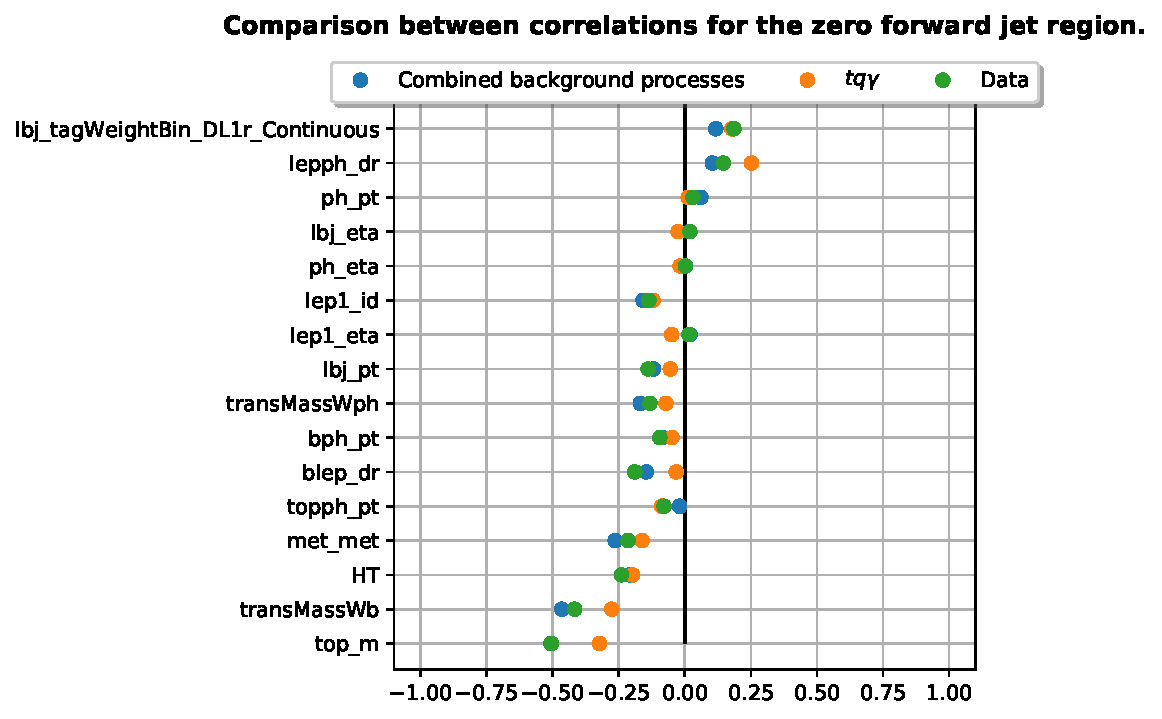
\includegraphics[width=0.7\textwidth]{Plots/corr0fjvariables.pdf}
    \caption{Visualisation of the correlations of input variables with the NN output in the $0\,fj$ region for the background samples, $tq\gamma$ and the measured data.}
    \label{fig:corr0fj}
\end{figure}
\begin{figure}
    \centering
    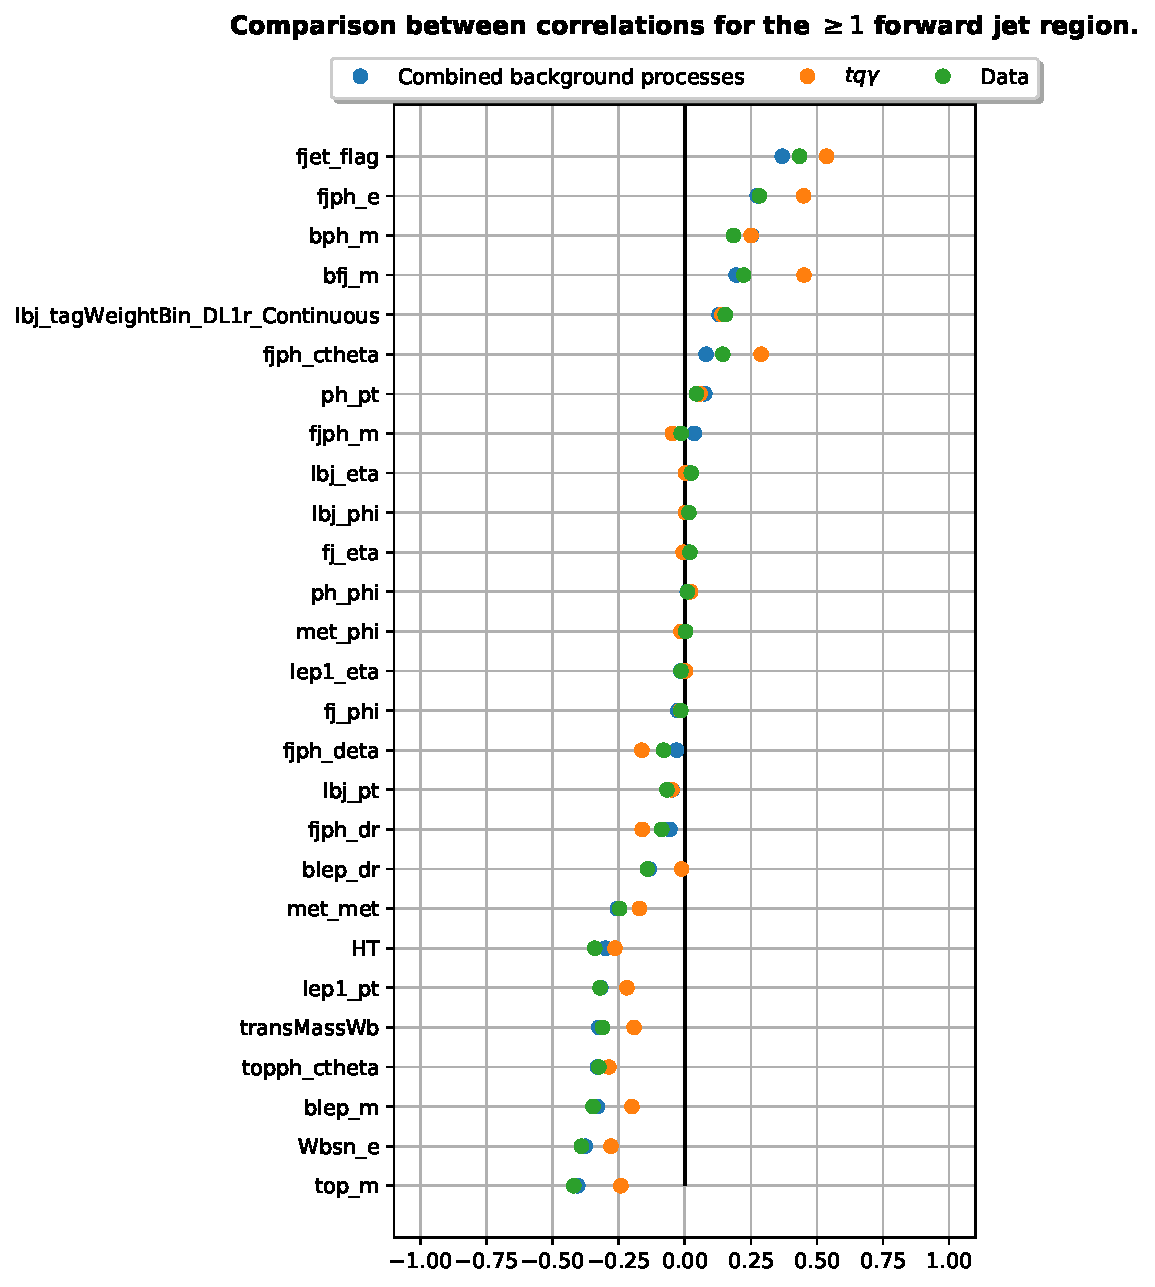
\includegraphics[width=0.7\textwidth]{Plots/corr1fjvariables1.pdf}
    \caption{Visualisation of the correlations of input variables with the NN output in the $\geq 1\,fj$ region for the background samples, $tq\gamma$ and the measured data.}
    \label{fig:corr1fj}
\end{figure} 

\section{NN output distribution dependence on photon \texorpdfstring{$p_T^\gamma$}{pTGamma} and fjet+photon energy \texorpdfstring{$E_{fj\text{+}\gamma}$}{}}
\label{sec:dependence}

In this section, two input variables are chosen to analyse the influence on the NN output further. In the first part of the analysis, an energy region for the input variables is chosen. Then, only events within that energy region are considered. This will be referred to as a "cut" throughout this section. 
After the cut, the distribution of the NN output is plotted to determine any noticeable changes. Additionally, a threshold for the NN output is chosen, and events above the threshold are examined. The $tq\gamma$ above the threshold must not exceed a statistical error $\frac{N_\text{signal}}{\sqrt{N_\text{signal}}}$ of over $10\%$. 
The composition of events above the threshold is then visualised and discussed. Finally, changes in signal and background compositions are examined. For simplicity and better sensitivity, only the $\geq 1$ forward jet region is considered in this analysis.

To compare with the NN output before any cut is applied, the Figure~\ref{fig:full} gives the composition of the NN output for two different threshholds. One at $NN = 0.9$ and the other at the highest possible threshhold before the statistical error becomes too high. The same thresholds are used in other composition plots of this analysis. 

The first input variable that is to be analysed is the photon's transverse momentum $p_T^\gamma$. As the $tq\gamma$ process is sensitive to the top quark to photon coupling, analysing the output dependence of the momentum of the photon provides an excellent way to test this prediction. 
The distribution of $p_T^\gamma$ is shown in \autoref{fig:ph_pt}. 

Results from \autoref{sec:corrvis} give a low correlation of $p_T^\gamma$ at around $5.8\%$ for the $tq\gamma$ sample in the $\geq 1\, fj$ region. The dependence of the NN output on $p_T^\gamma$ is therefore found not to be significant. 
With the help of the distribution, it is chosen to cut $p_T^\gamma$ at $40\,\si{\giga\electronvolt}$. The positive correlation predicts that higher values for $p_T^\gamma$ result in a better signal-background discrimination in the NN output. 
The NN output distribution for events with $p_T^\gamma \geq 40\,\si{\giga\electronvolt}$ is displayed in \autoref{fig:outputA40ph}. The composition after two different threshholds is shown in \autoref{fig:phptA40}.

When comparing Figures \ref{fig:NNdistro} and \ref{fig:outputA40ph} it is noticeable that $S/B$ does increase for higher values of $p_T^\gamma$ but the different is not significant and is not examined further. 
More noticeable differences are seen when comparing Figures \ref{fig:full} and \ref{fig:phptA40}. Here, it can be clearly seen that the parcentage of $t\bar{t}$ in the background is substantially higher (jumps from $35.8\%$ to $47.8\%$). 
This suggests that the $t\bar{t}$ has a $p_T^\gamma$ for the falsely reconstructed photon of this process. Without a deeper analysis, no more statements can be made on this incident. 
In addition, the contributions of less signfiicant background processes, which are depicted in the category "other", do get suppressed. The $38.8\%$ background contribution of this category falls to $26\%$ for the $p_T^\gamma$ cut.

The second input variable is the sum of the photon and forward jet energies $E_{fj\text{+}\gamma}$. This input feature has the second most strongest correlation with the NN output for the signal sample at around $44.99\%$. 
Because of its high correlation, $E_{fj\text{+}\gamma}$ is an important candidate variable that may be essential in the understanding of the top+photon coupling. It is also important to analyse a strongly correlated variable alongside a weakly correlated variable to test nature of the NN output and variables at different limits.

The distribution of $E_{fj\text{+}\gamma}$ is shown in \autoref{fig:fjph_e}. $E_{fj\text{+}\gamma}$ is chosen to be cut to the region $E_{fj\text{+}\gamma} \geq 900\,\si{\giga\electronvolt}$. 
The high positive correlation of $E_{fj\text{+}\gamma}$ predicts a greater discrimination between signal and background for larger energy values the variable. This is verified by the NN output distribution after the cut in 
\autoref{fig:outputA900fjph_e}. It is clear that the $S/B$ ratio is signficiantly higher for $NN > 0.5$. These results confirm that strongly correlated variables have stronger influences on the signal-background discrimination of the NN.
The composition of the events above the two different threshholds is depicted in \autoref{fig:fjph_eA900comp}. Here, there is no significant change seen in the composition of the main background as it was the case with the cut on $p_T^\gamma$. 


\begin{figure}
    \centering
    \begin{subfigure}[b]{0.6\textwidth}
       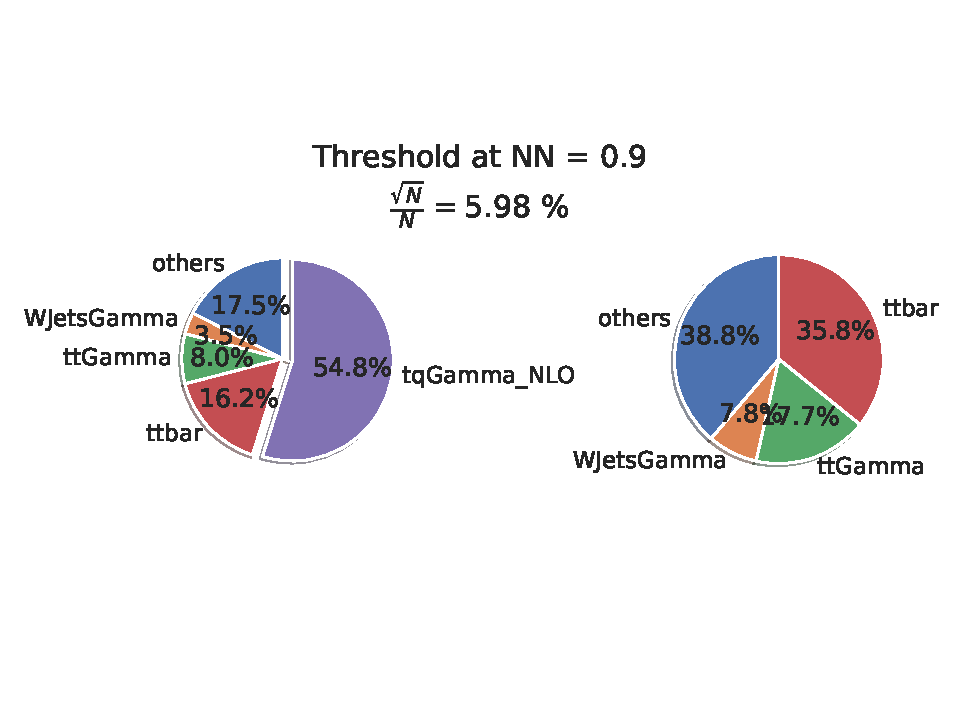
\includegraphics[width=1\linewidth]{Plots/composition9FULL.pdf}
    \end{subfigure}
    
    \begin{subfigure}[b]{0.6\textwidth}
       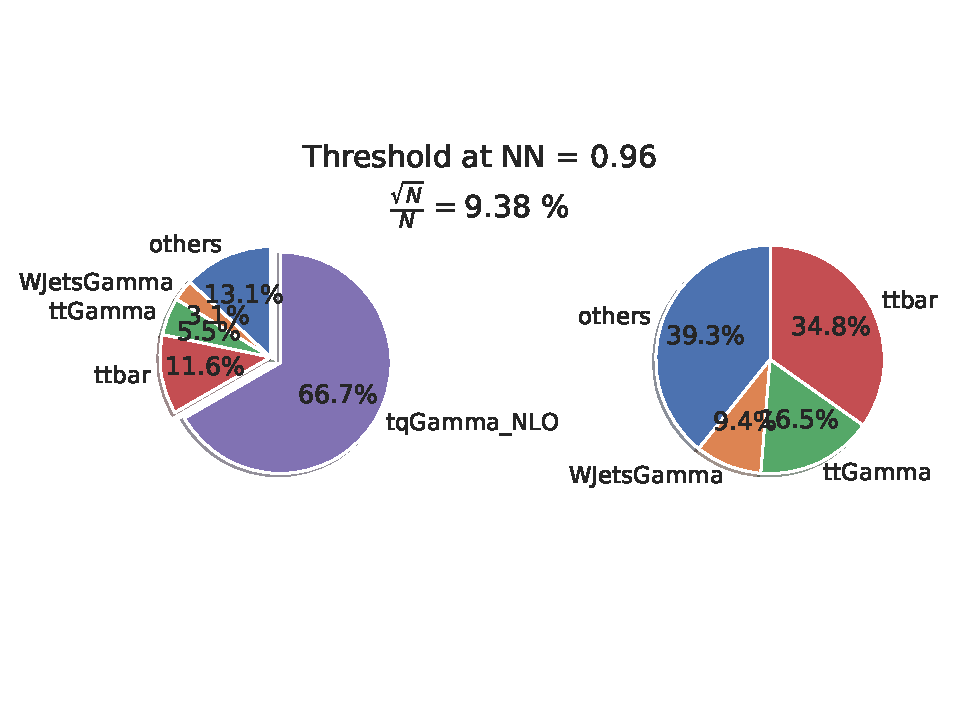
\includegraphics[width=1\linewidth]{Plots/compositionTenFULL.pdf}
    \end{subfigure}
    \caption{Composition of NN output for two different threshholds without any cuts applied. The right pie chart gives the composition without of the background.}
    \label{fig:full}
\end{figure}


\begin{figure}
    \centering
    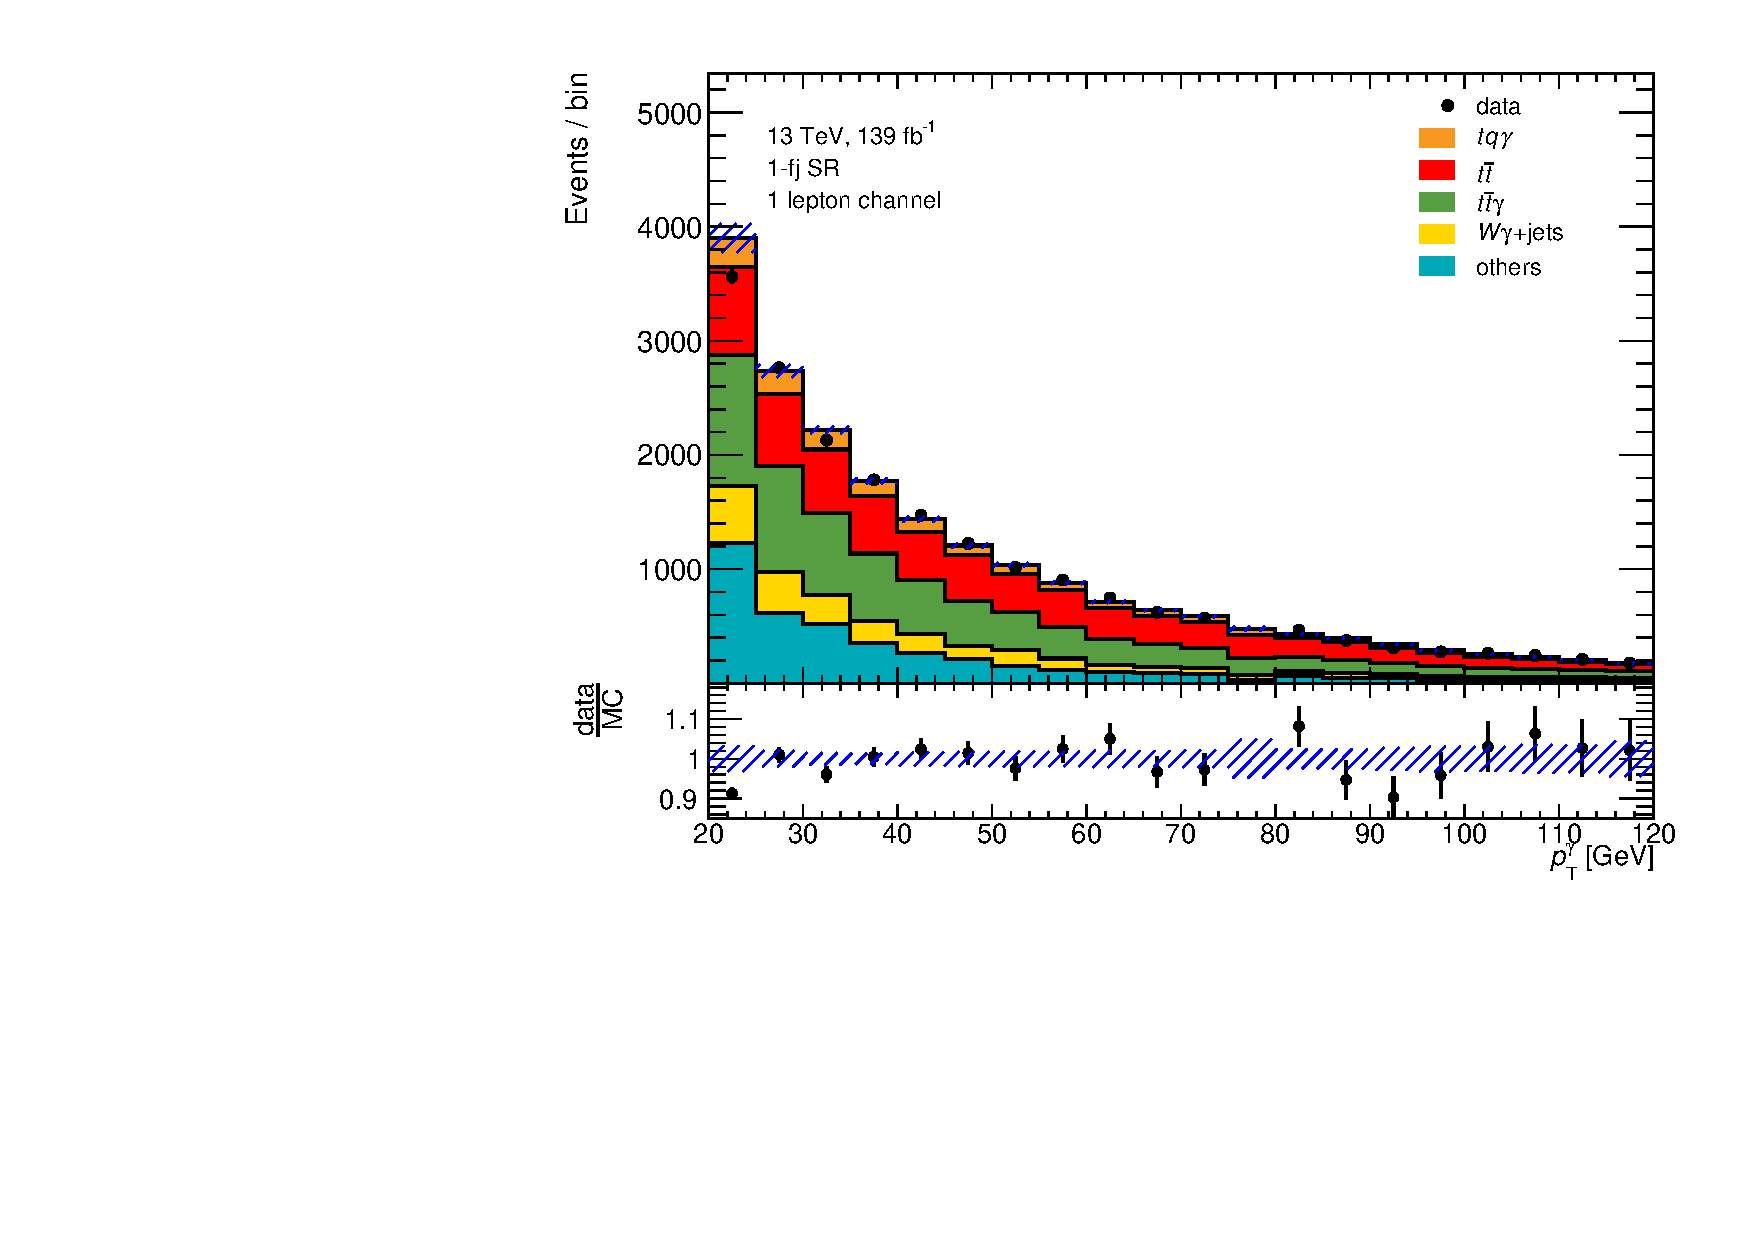
\includegraphics[width=0.6\textwidth]{Plots/ph_pt.pdf}
    \caption{Distribution of the transverse momentum of the photon $p_T^\gamma$.}
    \label{fig:ph_pt}
\end{figure}

\begin{figure}
    \centering
    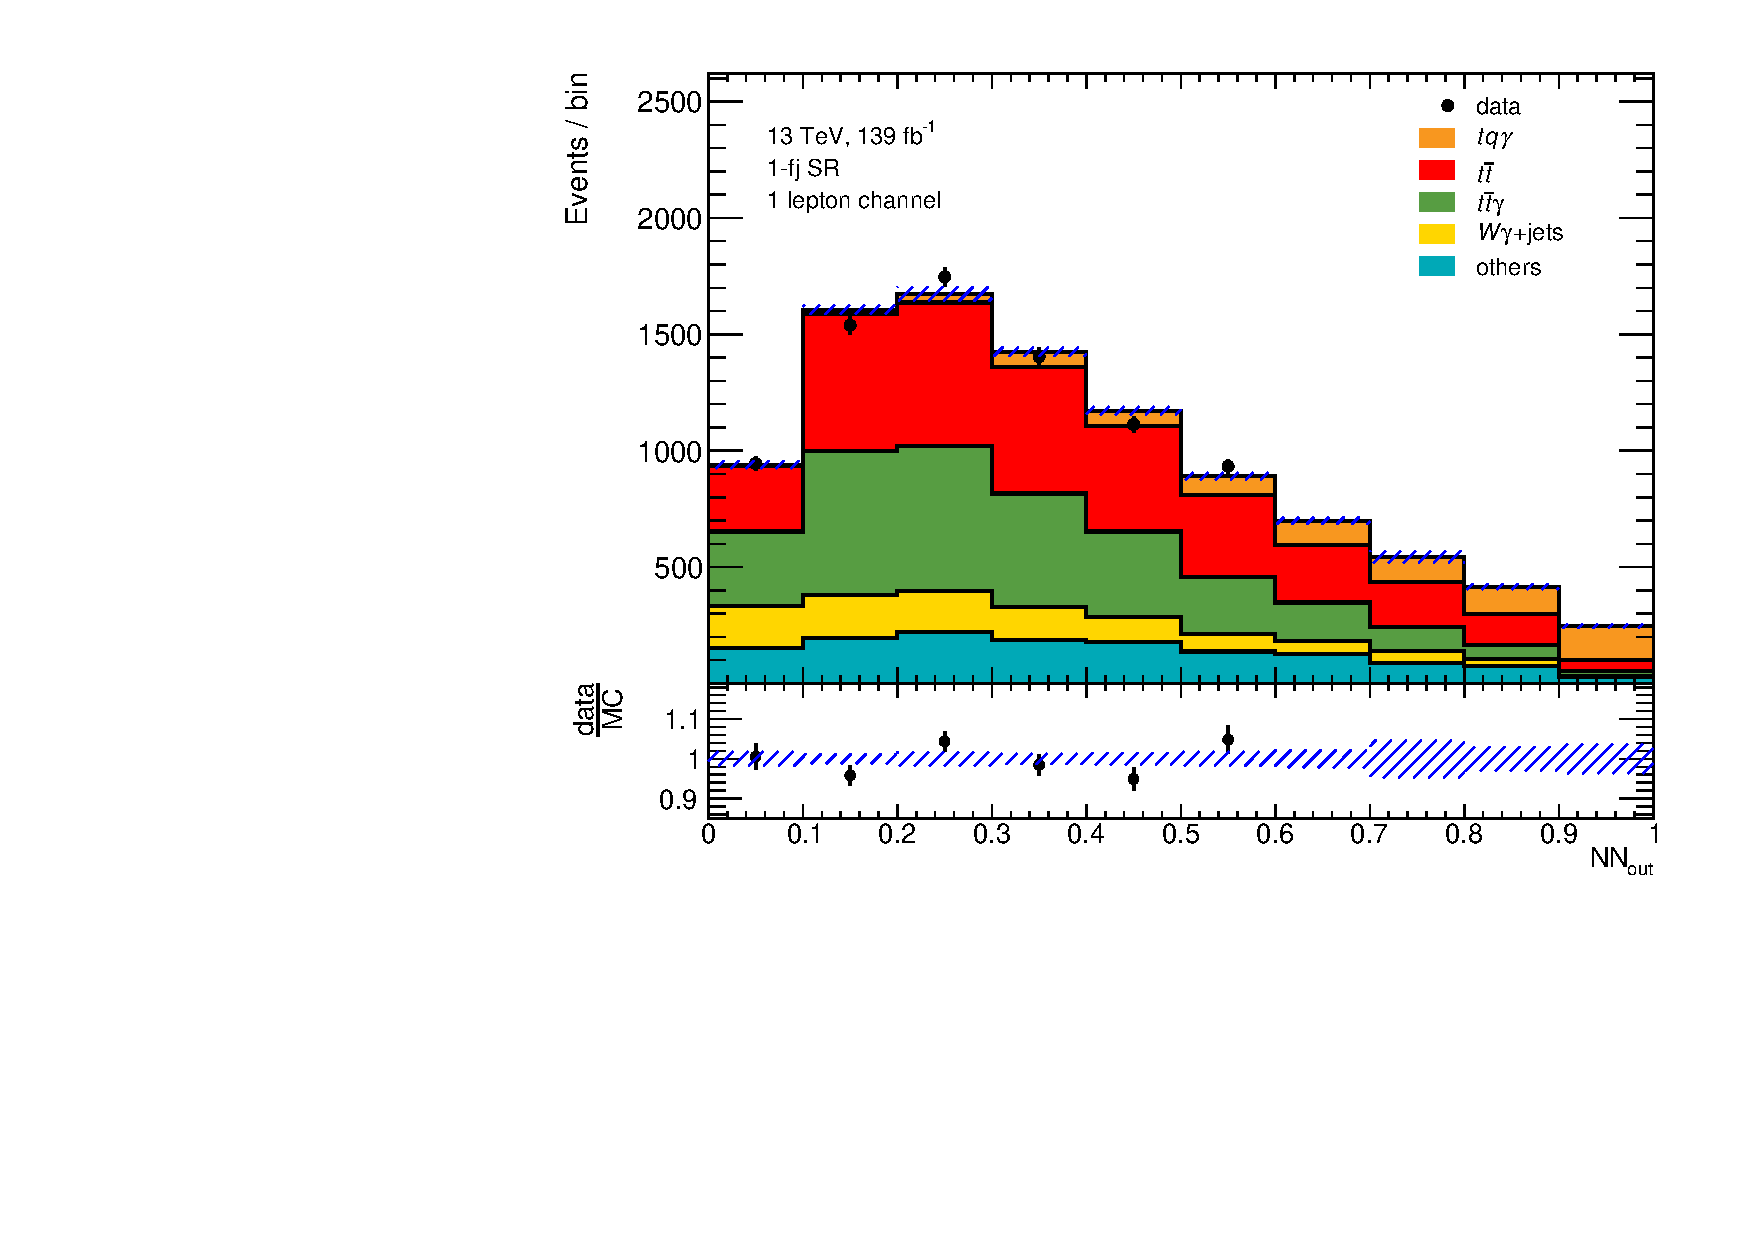
\includegraphics[width=0.7\textwidth]{Plots/NN_out_mixphA40.pdf}
    \caption{NN output distribution for the $p_T^\gamma \geq 40\,\si{\giga\electronvolt}$ region.}
    \label{fig:outputA40ph}
\end{figure} 

\begin{figure}
    \centering
    \begin{subfigure}[b]{0.6\textwidth}
       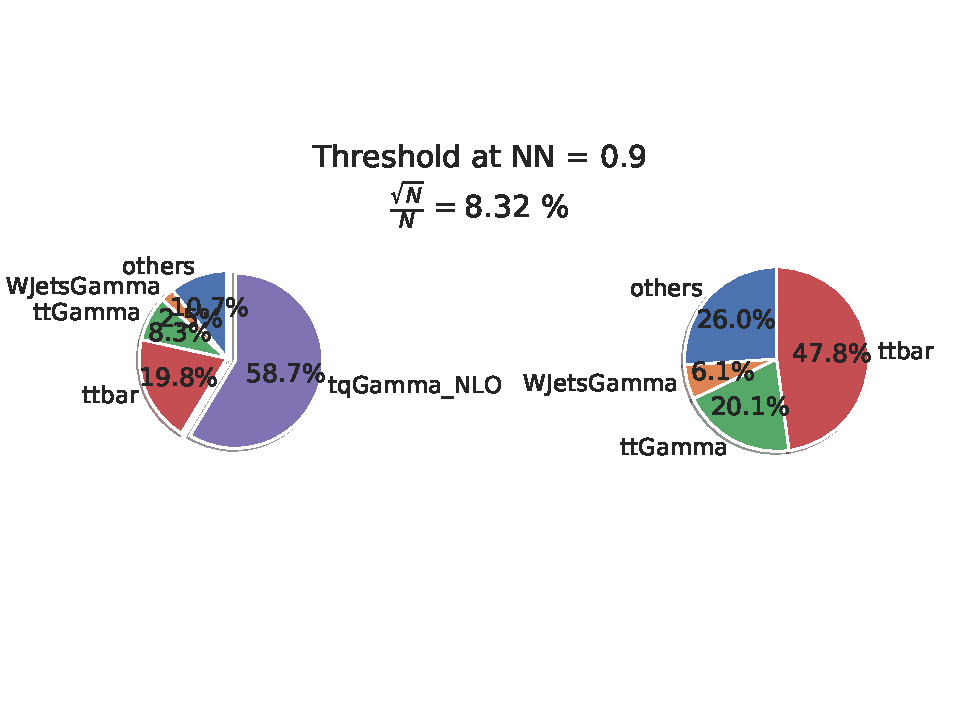
\includegraphics[width=1\linewidth]{Plots/composition9phA40.pdf}
    \end{subfigure}
    
    \begin{subfigure}[b]{0.6\textwidth}
       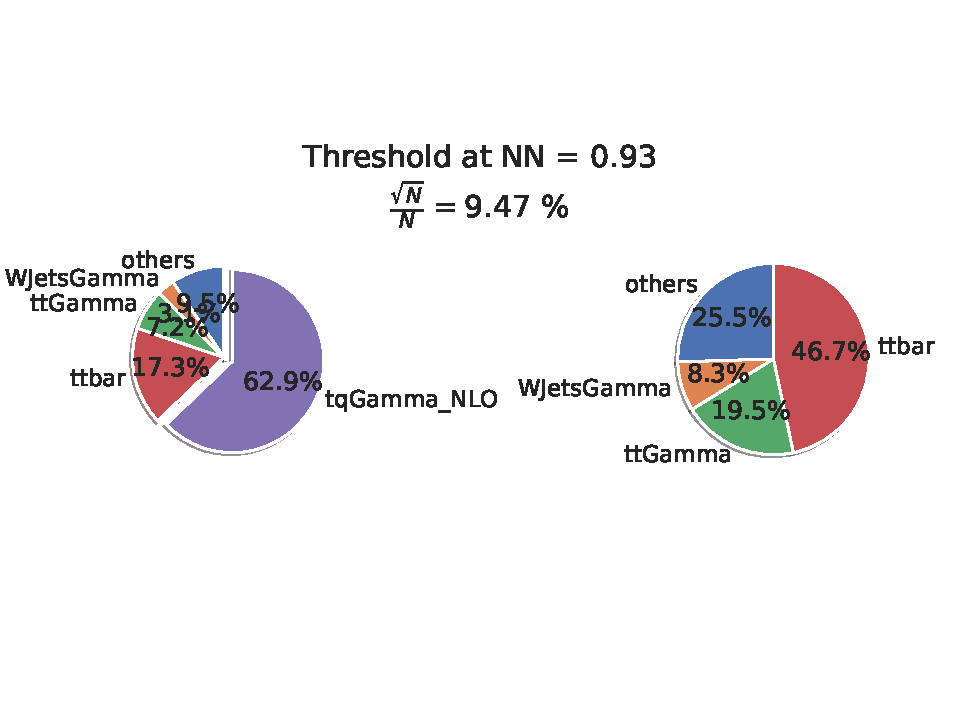
\includegraphics[width=1\linewidth]{Plots/compositionTenphA40.pdf}
    \end{subfigure}
    \caption{Composition of NN output for two different threshholds in the region $p_T^\gamma \geq 40\,\si{\giga\electronvolt}$. }
    \label{fig:phptA40}
\end{figure}

\begin{figure}
    \centering
    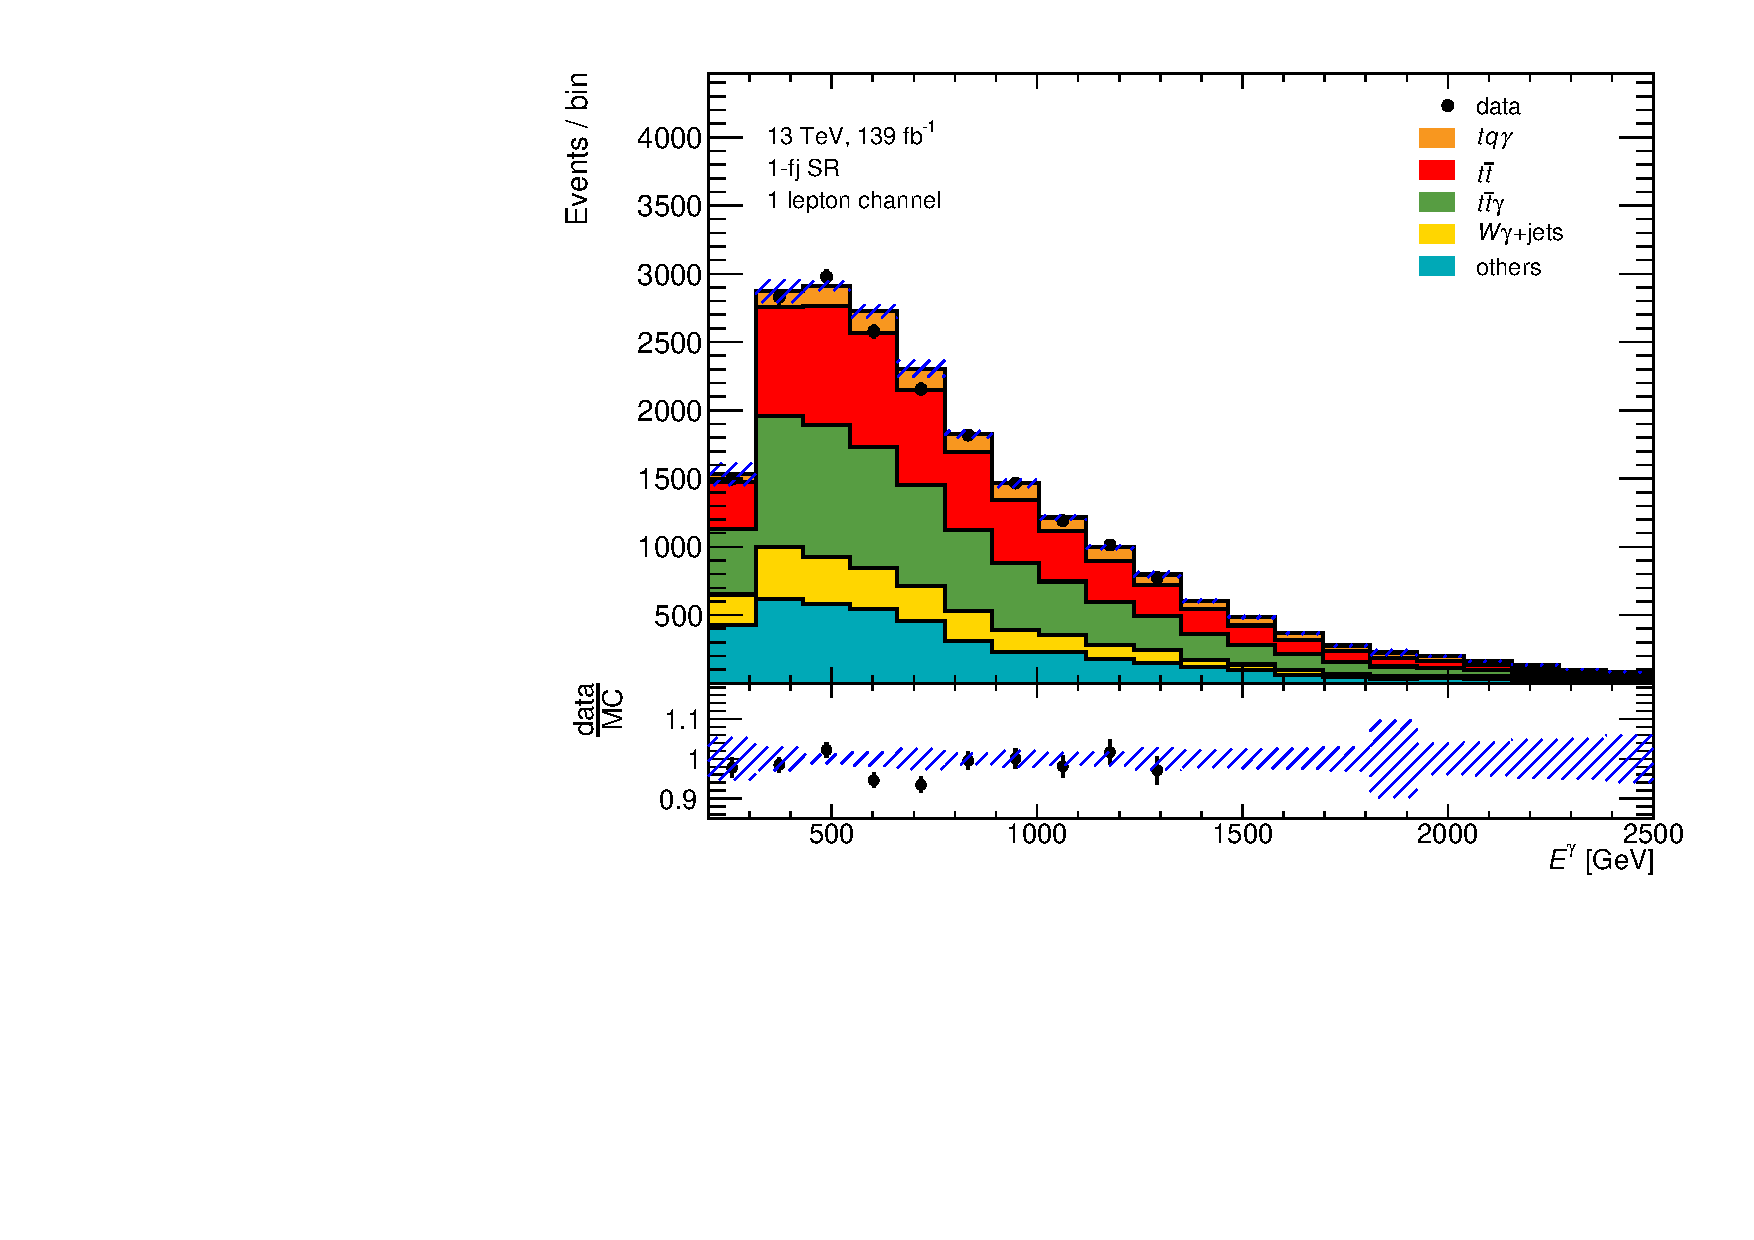
\includegraphics[width=0.7\textwidth]{Plots/fjph_e.pdf}
    \caption{Distribution of the forward jet + photon energy $E_{fj\text{+}\gamma}$.}
    \label{fig:fjph_e}
\end{figure} 


\begin{figure}
    \centering
    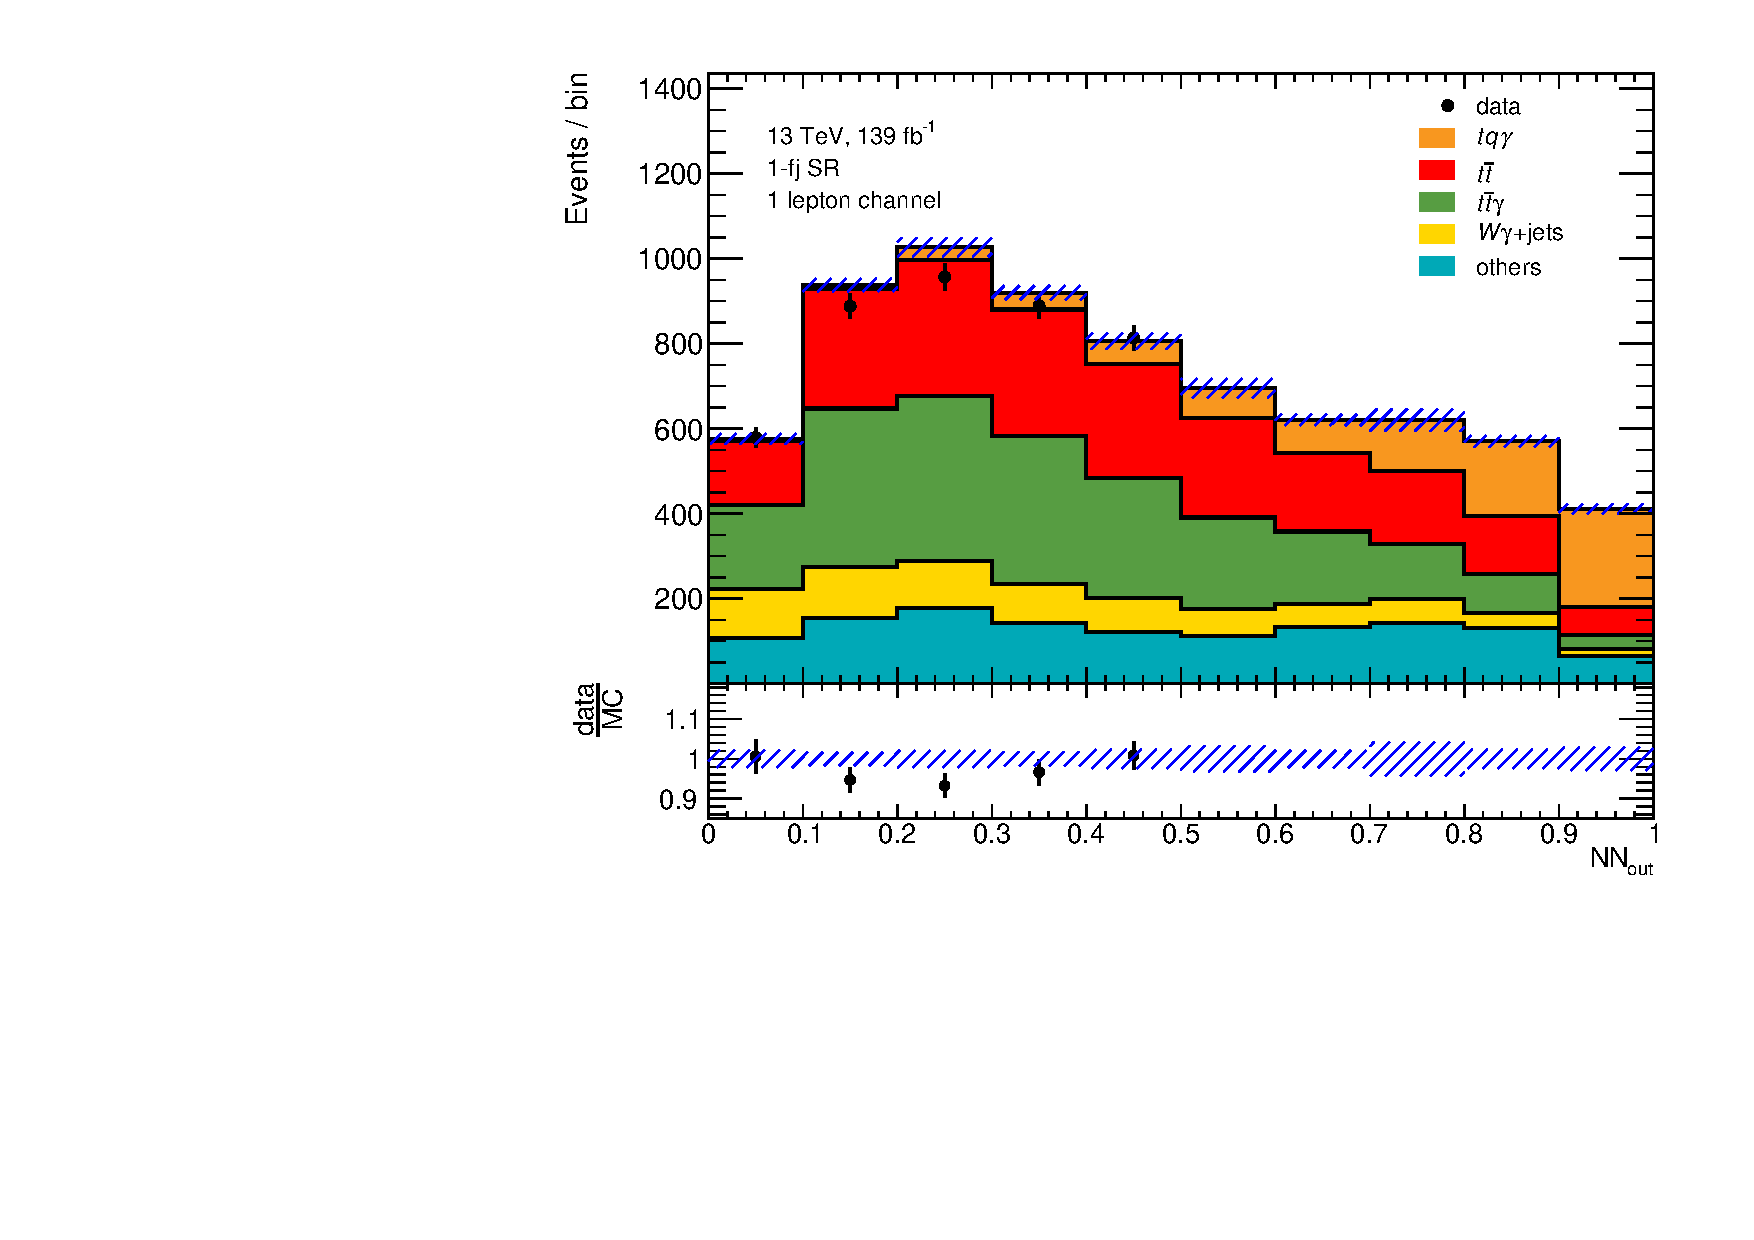
\includegraphics[width=0.7\textwidth]{Plots/NN_out_mixfjphA900.pdf}
    \caption{NN output distribution for the $E_{fj\text{+}\gamma} \geq 900\,\si{\giga\electronvolt}$ region.}
    \label{fig:outputA900fjph_e}
\end{figure} 

\begin{figure}
    \centering
    \begin{subfigure}[b]{0.6\textwidth}
       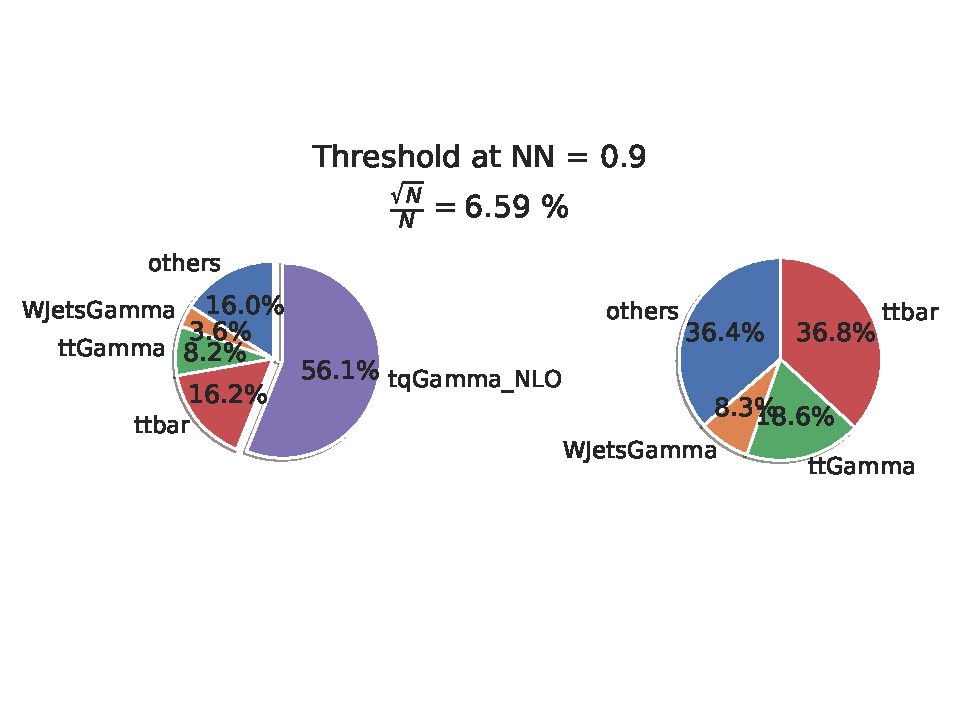
\includegraphics[width=1\linewidth]{Plots/composition9fjA900.pdf}
    \end{subfigure}
    
    \begin{subfigure}[b]{0.6\textwidth}
       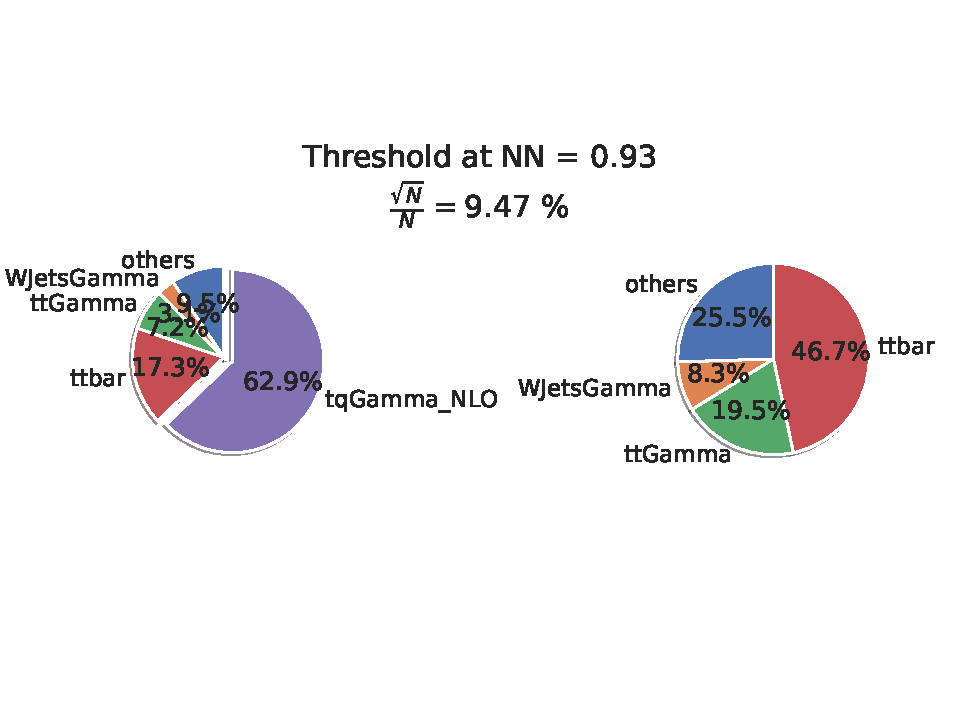
\includegraphics[width=1\linewidth]{Plots/compositionTenphA40.pdf}
    \end{subfigure}
    \caption{Composition of NN output for two different threshholds in the region $E_{fj\text{+}\gamma} \geq 900\,\si{\giga\electronvolt}$. }
    \label{fig:fjph_eA900comp}
\end{figure}